\documentclass{article}
\usepackage{iclr2026_conference,times}
% \iclrfinalcopy  % uncomment for camera-ready
\usepackage{amsmath,amssymb,amsthm}
\usepackage{graphicx}
\usepackage{booktabs}
\usepackage{tabularx}
\usepackage{microtype}
\usepackage[colorlinks=true,linkcolor=blue!60!black,citecolor=blue!60!black,
urlcolor=blue!60!black,hypertexnames=false]{hyperref}
\usepackage{xcolor}
\usepackage{enumitem}
\usepackage{algorithm,algorithmic}
\setlist{topsep=2pt,itemsep=1pt,leftmargin=1.4em}

\newtheorem{proposition}{Proposition}
\newtheorem{lemma}{Lemma}
\theoremstyle{remark}
\newtheorem{remark}{Remark}
\newenvironment{interp}{\par\vspace{2pt}\noindent\small\textbf{Interpretation.}\itshape}{\par\vspace{4pt}}
\newcommand{\takeaway}[1]{\par\vspace{3pt}\noindent\fcolorbox{black!20}{black!4}{\parbox{0.96\linewidth}{\small\textbf{Takeaway.} #1}}\vspace{4pt}}
\newcommand{\passat}[1]{\text{pass@}#1}

% float packing: relax LaTeX's conservative float fractions so figure
% pages fill and floats share pages with text
\renewcommand{\topfraction}{0.9}
\renewcommand{\bottomfraction}{0.6}
\renewcommand{\textfraction}{0.08}
\renewcommand{\floatpagefraction}{0.8}
\setcounter{topnumber}{3}
\setcounter{totalnumber}{5}

\title{The Estimator Decides: Finite-Group Activity, Curriculum\\
Allocation, and Hindsight Coverage in RL with Verifiable Rewards}
\author{Anonymous authors\\
Paper under double-blind review}

\begin{document}
\maketitle

\begin{abstract}
Difficulty curricula and hindsight relabeling are often treated as
objective-agnostic modules for reinforcement learning with verifiable
binary rewards. We show that their effect depends on the finite-group
estimator underneath. For the practical centered MaxRL implementation
that drops all-fail groups, a prompt with pass rate $p$ and $N$ rollouts
has expected coefficient mass
$A_N(p)=2[(1-p)-(1-p)^N]$. Its expected update factorizes as
$\mathbb E[\widehat g\mid x]=\tfrac12A_N(p)(\mu_+-\mu_-)$, so the
normalized mass is exactly the estimator-controlled scalar multiplying
the success-versus-failure score separation. Its shape and unique peak
are set by $N$, motivating a prompt sampler without a hand-set target
difficulty. The result is implementation-specific: raw MaxRL and the
full control-variate variant target order $N$, whereas the deployed
drop-all-fail estimator targets order $N-1$; the full variant assigns
negative coefficients when every rollout fails. In a matched-budget
20-seed tabular control, that alternative invokes the update callback for
every all-fail group but
does not reliably bootstrap the frontier (its median rounds to zero), while
verified hindsight reaches $0.927\pm0.003$ AUC. Relabeling, however, produces a
verified destination-conditioned update under a source-induced proposal,
not generally an on-policy destination gradient. In historical Countdown
runs, three-seed aggregate endpoints for a legacy per-trace relabeler show
higher mean success and lower $\passat{16}$ coverage; its saturation gate has one
promising but unintended moderate operating point. Historical maze runs use
a legacy utility and isolated positive imitation updates. They show an
estimator-associated coverage separation, but neither neural suite
instantiates the proposed common-destination algorithm, and the maze's
unbalanced sampler mix and shared warm starts preclude a causal interaction
claim.
Together the theory and experiments delimit what allocation can change,
what relabeling can create, and why both mean success and $\passat{k}$
coverage must be reported.
\end{abstract}

\section{Introduction}

Post-training with binary verifiers is constrained by a simple event: a
centered group update needs reward contrast. If all $N$ rollouts fail or
all $N$ succeed, the practical drop-constant-group estimator is silent.
This finite-group fact is not visible in a population weight function,
which describes a prompt only after averaging over sampling. A curriculum
acts one step earlier, deciding which prompts receive the rollout budget
needed to make those weights observable.

The field's response is a pair of data-level interventions. The first is
the \emph{difficulty curriculum}: reallocate the rollout budget toward
tasks where learning is possible right now --- UCB bandits over
difficulty buckets \citep{dump}, target-difficulty controllers
\citep{adarft}, category bandits \citep{sec}, learnability-based
rejection sampling \citep{lilo}, dead-prompt filtering \citep{dapo,greso}.
The second is \emph{failure recycling}: relabel a failed rollout as a
verified example of an achieved destination \citep{her,gcsl,lfh,hir}.
Both interventions are often evaluated as estimator-agnostic modules,
and mainly with mean accuracy. That can miss two distinct questions:
whether the deployed estimator produces a usable finite-group update,
and whether concentrating updates changes multi-sample coverage.

We study these questions through the exact finite-group coefficient
profile of the estimator actually deployed. For practical centered
MaxRL, its normalized coefficient mass has two endpoint zeros and one
interior maximum. These induce three \emph{operational}, budget-dependent
regimes: negligible contrast, a frontier of high estimator activity, and
a saturated tail. The profile constrains local activity; it does not by
itself determine cross-task transfer or final performance. Three questions
organize the paper:

\emph{Q1: What activity profile does the estimator implement?} For the
practical centered/drop estimator, the expected coefficient mass is
$A_N(p)=2(\passat{N}-\passat{1})$ and the expected update factorizes into
$A_N/2$ times the success-versus-failure score separation
(\S\ref{sec:theory}). The curve's shape and exact peak follow from $N$;
under our normalization, its $N{=}2$ case is the $p(1-p)$ learnability
score used by prior curricula. Raw MaxRL and full-control-variate MaxRL
have different activity profiles, so the result belongs to the deployed
implementation, not to every estimator bearing the MaxRL name.

\emph{Q2: What can allocation and relabeling change?} Reallocation cannot
manufacture a positive anchor for an all-fail group under the practical
estimator. The full control-variate estimator is an important
counterexample at the sample level: it assigns a negative-only coefficient
vector and invokes the update path there.
We therefore test it directly rather than claim impossibility. Hindsight
can instead create verified destination contrast, but its data are drawn
from a source-induced proposal and are generally off-policy for the
destination (\S\ref{sec:recycling}). Historical Countdown runs used a
different, per-trace relabeler; their three-seed aggregate endpoints show
higher mean accuracy and lower $\passat{k}$ coverage, a descriptive pattern we call
\textbf{recycling-induced sharpening} rather than validation of the proposed
destination-group estimator.

\emph{Q3: Can destination saturation control that trade?} The mastered
endpoint motivates rejecting relabels to already-reachable destinations.
We instantiate this with a tuned pass-rate threshold. At an unintended
moderate effective strength, the three-seed frontier-coverage point estimate
returns near baseline while retaining part of the mean-gain point estimate;
the corrected stronger setting is only a
single-seed endpoint and is reported as preliminary (\S 6.9). Thus the
algebra motivates the admission variable, while the operating threshold
remains empirical.

Our contributions:
\begin{enumerate}
\item \textbf{Finite-group theory.} We distinguish raw, full-control-
  variate, and practical MaxRL; derive the practical estimator's exact
  coefficient-mass profile and update factorization; and show that its
  drop-all-fail convention corresponds to truncation order $N-1$.
\item \textbf{Allocation and recycling.} We use normalized coefficient
  mass as a prompt-sampling utility and characterize hindsight as a
  verified but generally off-policy destination semi-gradient.
\item \textbf{Missing-control evidence.} A matched-budget 20-seed CPU
  experiment shows that the full-control-variate all-fail coefficient
  branch does not reliably unlock the frontier-heavy pool, whereas exact relabeling
  does. A separate fixed-schedule control with disjoint tuning and held-out
  evaluation seeds
  puts practical MaxRL, GRPO, and RLOO within $0.005$ AUC on the balanced
  exact-score pool.
\item \textbf{Coverage effects and boundaries.} Legacy Countdown runs
  report a three-seed aggregate mean-versus-$\passat{k}$ cost for their per-trace relabeler;
  a saturation gate is promising but preliminary. Maze and LLM runs are
  retained as explicitly implementation-mismatched diagnostics, while
  locomotion and Jugs mark further evidence limits.
\end{enumerate}
The order-$N-1$ result refines the implementation-level reading of MaxRL
Algorithm 1; it does not contradict the order-$N$ theorem for the raw or
full-control-variate estimators. Negative results and retractions are
reported in place (\S\ref{sec:limits}).

\begin{figure}[t]
\centering
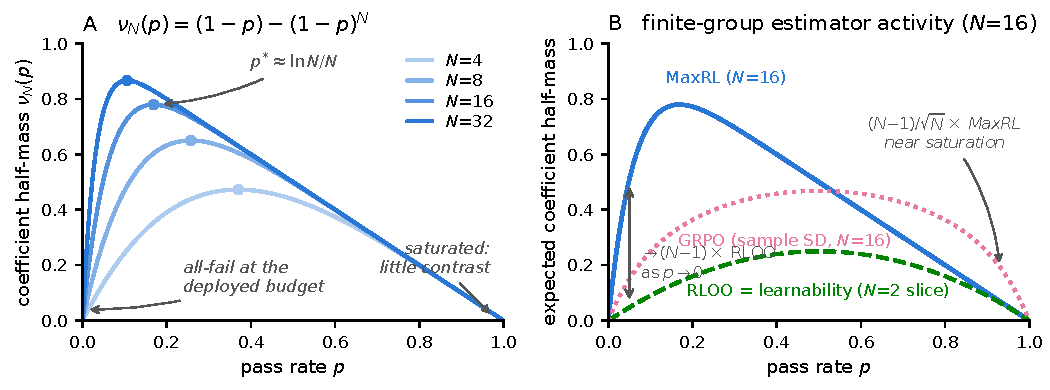
\includegraphics[width=\linewidth]{figures/fig1_utility}
\caption{\textbf{Finite-group estimator activity.} \emph{Left:} normalized
coefficient mass $\nu_N(p)=(1-p)-(1-p)^N$ for the practical centered/drop
estimator. Its exact peak is $p^*=1-N^{-1/(N-1)}$; low activity near an
endpoint is operationally important only relative to the deployed budget.
\emph{Right:} expected coefficient half-mass at $N{=}16$. The GRPO curve
uses the code's sample-standard-deviation convention (fixed $10^{-6}$
stabilizer included), not the population-SD limit. The following endpoint
ratios take the zero-stabilizer limit, as in Proposition~\ref{prop:ratio};
the stabilizer changes no plotted digit. As $p\to0$, practical
MaxRL/RLOO tends to $N-1$ and practical MaxRL/GRPO tends to $\sqrt N$;
as $p\to1$, MaxRL and RLOO both decay linearly while GRPO/MaxRL tends to
$(N-1)/\sqrt N$. Under our normalization, RLOO is proportional to the
$p(1-p)$ learnability score used by SFL and LILO.}
\label{fig:utility}
\end{figure}

\section{From MaxRL objectives to finite-group activity}
\label{sec:theory}
For a prompt \(x\) and group size \(N\ge2\), let
\(r_i\in\{0,1\}\), \(K=\sum_{i=1}^N r_i\),
\(p=\Pr(r=1\mid x)\), \(q=1-p\), and
\(S_i=\nabla_\theta\log\pi_\theta(z_i\mid x)\). MaxRL truncates
\(\log p=-\sum_{t\ge1}q^t/t\) at
\[
J_T(p):=-\sum_{t=1}^{T}\frac{q^t}{t}.
\]
The baseline paper separates a raw estimator from its control-variate
form; its practical algorithm adds a further constant-group convention.
Those three choices have different finite-group activity profiles:
\begin{align}
H_N &:= \mathbf 1\{K>0\}\frac1K\sum_i r_iS_i,
&&\text{raw success average}, \\
C_N &:= H_N-\frac1N\sum_iS_i,
&&\text{full control variate}, \\
D_N &:= \mathbf 1\{K>0\}
 \left(\frac1K\sum_i r_iS_i-\frac1N\sum_iS_i\right),
&&\text{practical centered/drop}.
\end{align}

\begin{table}[t]
\centering\small
\caption{\textbf{Three MaxRL estimators.} Mass is expected total
absolute score coefficient, \(A(p)=\mathbb E\sum_i|w_i|\). The order-\(N-1\)
statement applies only to the practical convention that drops the whole
all-fail group.}
\label{tab:estimators}
\begin{tabular}{@{}lccc@{}}
\toprule
estimator & \(K=0\) sample update & target & coefficient mass \(A(p)\) \\
\midrule
raw \(H_N\) & \(0\) & \(J_N\) & \(1-q^N\) \\
full CV \(C_N\) & \(-N^{-1}\sum_iS_i\) & \(J_N\) & \(2q-q^N\) \\
practical \(D_N\) & \(0\) & \(J_{N-1}\) & \(2(q-q^N)\) \\
\bottomrule
\end{tabular}
\end{table}

Tajwar et al.'s order-\(N\) theorem is exact for \(H_N\), and the
zero-mean control variate leaves \(C_N\) unbiased for the same target
\citep{maxrl}. The next lemma concerns only the additional drop rule in
the shipped practical loop.

\begin{lemma}[Order of the practical drop estimator]
\label{lem:trunc}
The practical estimator \(D_N\) is unbiased for \(J_{N-1}\), not \(J_N\).
\end{lemma}
\begin{proof}
Relative to \(C_N\), zeroing the control variate only on \(K=0\) removes
an expected \(q^{N-1}\nabla p\). Hence
\[
\mathbb E[D_N\mid x]
=\left(\sum_{j=0}^{N-1}q^j-q^{N-1}\right)\nabla p
=\sum_{j=0}^{N-2}q^j\nabla p
=\nabla J_{N-1}(p).
\]
\end{proof}
This is an implementation-level refinement, not a correction of the raw
estimator theorem.

\begin{proposition}[Coefficient mass and exact update factorization]
\label{prop:mass}
For \(0<p<1\), define
\[
\mu_+(x)=\mathbb E[S\mid r=1,x]=\frac{\nabla p}{p},
\qquad
\mu_-(x)=\mathbb E[S\mid r=0,x]=-\frac{\nabla p}{q}.
\]
For the practical estimator,
\begin{equation}
\boxed{
A_N(p):=\mathbb E\sum_i|w_i|=2\nu_N(p),\qquad
\nu_N(p):=q-q^N=\passat{N}(p)-p,
}
\label{eq:mass}
\end{equation}
and
\begin{equation}
\boxed{
\mathbb E[D_N\mid x]
=\nu_N(p)(\mu_+-\mu_-)
=\frac{\nu_N(p)}{pq}\nabla p
=\sum_{j=0}^{N-2}q^j\nabla p.
}
\label{eq:factor}
\end{equation}
\end{proposition}
\begin{proof}
Conditioned on \(K=k>0\), the positive coefficients sum to
\(1-k/N\), and the negative coefficients have the same absolute sum.
Thus the conditional coefficient mass is \(2(1-k/N)\) and the
conditional expected update is
\((1-k/N)(\mu_+-\mu_-)\). Averaging over \(K\sim\mathrm{Bin}(N,p)\)
gives
\(\mathbb E[(1-K/N)\mathbf 1\{K>0\}]=1-q^N-p=q-q^N\).
Finally, \(\mu_+-\mu_-=\nabla p/(pq)\).
\end{proof}

Equation~\ref{eq:factor} gives \(\nu_N\) a precise interpretation: it is
the estimator-controlled scalar multiplying the success-versus-failure
score separation. It is not the entire gradient geometry. Its unique
maximum is
\[
p^\star=1-N^{-1/(N-1)}\approx \frac{\log N}{N},
\]
and its endpoint zeros induce operational regimes rather than
mathematically fixed-width bands. If a task receives \(B\) groups, its
expected number of nonconstant groups is
\[
B\,[1-p^N-q^N].
\]
We call it operationally inactive at budget \((B,N)\) when this quantity
is much smaller than one. At \(p>0\), increasing \(B\) or \(N\) can move
the task out of that regime; at \(p=0\), reallocation under the same
policy and verifier cannot produce a success.

\begin{proposition}[Finite-group comparisons]\label{prop:ratio}
Under the coefficient conventions used here, RLOO has normalized
half-mass \(\nu^{\mathrm{RLOO}}(p)=pq\), so
\(\nu_N/\nu^{\mathrm{RLOO}}\to N-1\) as \(p\to0\), while both decay as
\(q\) when \(p\to1\). For the deployed sample-standard-deviation GRPO
implementation,
\begin{equation}
\nu_N^{\mathrm{GRPO}}(p)
=\mathbb E\!\left[
\frac{K(N-K)}
 {N^2\{\sqrt{K(N-K)/(N(N-1))}+\epsilon\}}
\right],
\label{eq:grpo-sample}
\end{equation}
with constant groups contributing zero. At \(\epsilon=0\), this is
\(\sqrt{(N-1)/N}\,N^{-1}\mathbb E\sqrt{K(N-K)}\), giving
\[
\frac{\nu_N}{\nu_N^{\mathrm{GRPO}}}\to\sqrt N\quad(p\to0),
\qquad
\frac{\nu_N^{\mathrm{GRPO}}}{\nu_N}\to\frac{N-1}{\sqrt N}\quad(p\to1).
\]
\end{proposition}
The population-SD GRPO curve often used in objective analyses differs by
the finite-\(N\) factor above; Eq.~\ref{eq:grpo-sample} matches our code
and historical experiments. The \(10^{-6}\) stabilizer changes no
reported digit at the group sizes studied.

\begin{proposition}[One-step fixed-rate allocation]\label{prop:alloc}
Suppose current task pass rates \(p_i\) are known and held fixed, task
\(i\) receives an integer group size \(n_i\ge1\), and
\(\sum_i n_i=B\). Greedy water-filling maximizes the separable one-step
objective \(\sum_i\nu_{n_i}(p_i)\): the marginal value of the next
rollout is
\[
\nu_{n_i+1}(p_i)-\nu_{n_i}(p_i)
=p_i(1-p_i)^{n_i},
\]
which decreases with \(n_i\).
\end{proposition}
This proposition is a mass-allocation oracle under fixed \(p_i\), not a
ceiling on sequential AUC or held-out performance. Policy change,
cross-task transfer, interference, posterior uncertainty, exploration
floors, and delayed skill unlocking all lie outside its assumptions. The
deployed teacher keeps a fixed group size and changes which prompt group
is drawn, using \(\nu_N^\gamma\) with a uniform floor.

\begin{remark}[Activity is not transfer]\label{rem:scope}
Equation~\ref{eq:factor} is exact for a prompt-local expected update, but
neither coefficient mass nor its endpoint zeros determine gradient norm,
cross-task transfer, or final performance. On the exact-score bridge,
\(\nu_N\) closely ranks first-order improvement
(\texttt{curriculum\_maxrl/results\_bridge.json}); later planning
experiments show that the best sequential index depends on whether the
target is anytime AUC or a final checkpoint. We therefore use
\(\nu_N\) as an estimator-aligned sampling score and test downstream
performance rather than treating it as a universal learning utility.
\end{remark}

\begin{remark}[Adaptive sampling changes the training distribution]
\label{rem:objective}
Conditioned on training history and treating selection as stop-gradient,
sampling prompts from \(q_t\) yields
\(\mathbb E_{x\sim q_t}[\nabla J(x)]\), not the data-distribution
gradient under \(\rho\) unless corrected. Because \(q_t\) adapts, these
updates are not generally the gradient of one fixed reweighted objective.
Evaluation definitions are fixed and method-independent under \(\rho\).
The exact-score controls reuse their task pool; disjoint tuning and
evaluation seeds are used where stated. Gym uses fixed task bins with fresh
episodes rather than a held-out task pool.
\end{remark}

The theory separates two interventions. Allocation changes \(q_t\) to
spend groups where the practical estimator is active. Hindsight changes
the conditioning and the destination proposal, potentially creating
verified contrast where the requested group has none. The latter falls
outside Proposition~\ref{prop:mass} and requires its own distributional
analysis.

\begin{figure}[t]
\centering
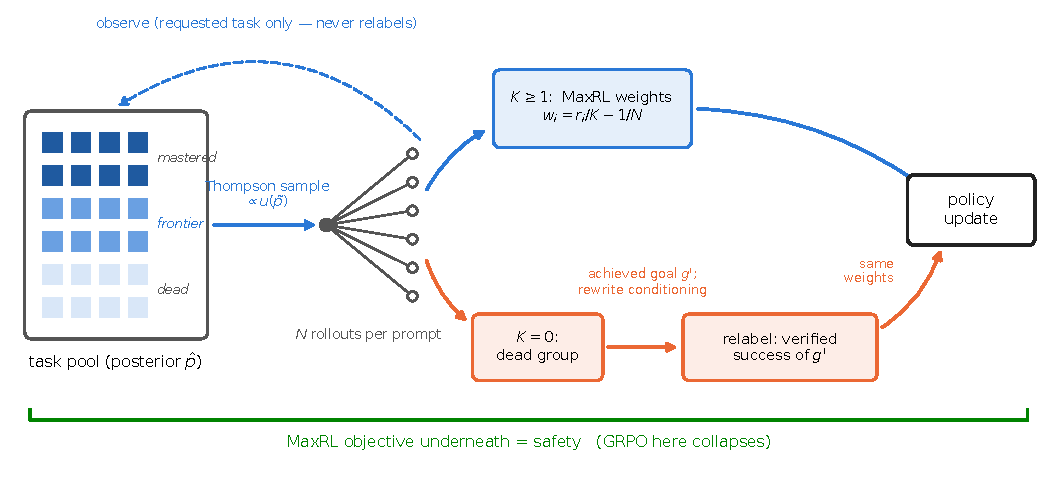
\includegraphics[width=\linewidth]{figures/fig4_algorithm}
\caption{\textbf{Proposed FrontierMax step.} The teacher samples requested
prompts by \(\nu_N\). A live requested group uses the practical estimator.
For an all-fail group, the relabeler selects one common destination,
rewrites and reverifies the group, and updates only if the destination
group has contrast \(0<K'<N\). The resulting update is verified but
generally off-policy for the destination. Posterior state is updated only
from requested-task outcomes.}
\label{fig:algorithm}
\end{figure}

\section{FrontierMax: estimator-aligned allocation}\label{sec:method}
FrontierMax is the corrected, proposed group-rollout loop whose teacher tracks requested-task
pass rates with decayed Beta state. Thompson sampling draws
\(\tilde p_x\) and samples prompt groups proportional to
\(\nu_N(\tilde p_x)^\gamma\), mixed with a uniform floor. Relabeled
outcomes never update the requested-task posterior; doing so inflated
\(\hat p\) from \(.47\) on evaluation to \(.81\) in a legacy maze control. The profile
\(\nu_N\), its peak, and its \(N\)-dependence are derived. Posterior decay,
the floor, concentration \(\gamma\), relabel dose, and gate threshold are
tuned controls (Table~\ref{tab:knobs}), not consequences of the theorem.

A per-prompt posterior is appropriate only when prompts recur enough to
accumulate evidence. At pools much larger than the number of groups, our
legacy-utility GSM8K pilot remains nearly uniform; a bucket posterior or learned
difficulty model is required at that scale. The current method claim is
therefore about repeated finite pools, with the large-pool result treated
as a delivery diagnostic.

\begin{algorithm}[t]
\caption{FrontierMax: one group step.}
\label{alg:frontiermax}
\begin{algorithmic}[1]
\STATE \(\triangleright\) sample requested prompts \(x_1,\ldots,x_B\)
  proportional to \(\nu_N(\tilde p_x)^\gamma\), with a uniform floor;
  \(\tilde p_x\sim\mathrm{Beta}(\alpha_x,\beta_x)\)
\STATE roll out \(N\) completions per prompt; verify requested rewards
  \(r_i\); set \(K=\sum_i r_i\)
\STATE update \((\alpha_x,\beta_x)\) from requested outcomes only
\STATE if \(0<K<N\), update with \(w_i=r_i/K-1/N\)
\STATE \(\triangleright\) if \(K=0\), choose one destination
  \(g'=H(x,z_{1:N})\); rewrite every conditioning to \(g'\)
\STATE reverify all rewritten trajectories under \(g'\), obtaining
  \(r'_i\) and \(K'=\sum_i r'_i\)
\STATE \(\triangleright\) admit only if \(0<K'<N\) and
  \(\hat p_{g'}\le\texttt{gate\_max\_p}\); recompute destination scores
  and use \(w'_i=r'_i/K'-1/N\)
\STATE update the policy from live requested groups and admitted
  destination groups
\end{algorithmic}
\end{algorithm}

Algorithm~\ref{alg:frontiermax}'s two defining pieces---the exact \(\nu_N\)
sampler and a common-destination, mixed-outcome relabeled group---are
instantiated together in the exact-score chain and in the corrected NumPy
interfaces. GridReach and Countdown regression-test the shared-destination
contrast explicitly; chain and Gym controls exercise relabeling without
asserting every contract in a dedicated regression.
The historical neural and LLM runs predate this contract: maze uses the
legacy \((1-q^N)q\) utility and per-trajectory positive-only recycling;
GSM8K uses the legacy utility; and Countdown combines that utility with
per-trace targets inside a uid group. Those runs are retained below as
diagnostics, not as end-to-end validation of Algorithm~\ref{alg:frontiermax}.

The gate is saturation-motivated, not parameter-free. With the
\(\mathrm{Beta}(1,1)\) initialization and threshold \(0.5\), an unseen
destination begins exactly on the admission boundary; the hard rule does
not model cold-start uncertainty. More conservative posterior bounds or
held-out destination probes are natural extensions.

\section{Failure recycling and proposal shift}\label{sec:recycling}

Let \(h_{\theta,g}(Z_{1:N})\) denote the practical destination update
after conditioning has been rewritten to \(g\) and every trajectory has
been reverified. Fresh destination groups follow
\[
P_{\theta,g}=\pi_\theta(\cdot\mid g)^{\otimes N},
\qquad
\nabla J_{N-1,g}=\mathbb E_{P_{\theta,g}}[h_{\theta,g}].
\]
Hindsight instead samples a source prompt \(x\), chooses a common
destination from the group, rewrites the group, and conditions on
admission. Let \(Q_{\theta,g}^{x\to g}\) be that induced proposal law.
Its expected update is
\[
U_g^{\mathrm{HS}}
=\mathbb E_{Q_{\theta,g}^{x\to g}}[h_{\theta,g}].
\]
Exact verification makes the label semantically valid; it does not make
\(Q_{\theta,g}^{x\to g}=P_{\theta,g}\). Equality of the two update moments
is necessary and sufficient for an exact fresh-destination gradient, and
equality of the laws is sufficient. Otherwise hindsight is a
distribution-shifted destination semi-gradient because the optimization
does not differentiate through the source proposal, destination choice,
or admission event. Same-group destination selection also breaks the
fixed-destination iid premise; selecting \(g\) with one group and updating
from a disjoint group is the clean cross-fitted control. This framing
matches the off-policy gap in GCSL and the corrected relabel distribution
derived by hindsight inference for policy improvement
\citep{gcsl,eysenbach}.

Three implementation contracts remain essential: \textbf{(1) semantic
verification} under the destination's exact verifier; \textbf{(2) one
common destination}, with every conditioning and score recomputed under
that destination; and \textbf{(3) destination contrast}, \(0<K'<N\).
The gridworld adapter and regression tests enforce rewriting and
reverification. An older no-rewrite comparison is described in project
notes, but its result artifact is not vendored and is therefore not used
quantitatively here. These behavioral contracts do not establish on-policy
exactness.

The historical fixed-pool placebo battery suggests that much of hindsight's
\(+0.22\) AUC gain is compatible with receiving an additional update:
live-gradient replay reaches \(0.832\), versus \(0.869\) for relabeling and
\(0.650\) for uniform training. The \(+0.037\) hindsight-minus-replay
difference is consistent across five seeds. However, the runs did not log
per-arm update counts or update norms, and the random-target arm reused a
stale reward vector with an unseeded random draw rather than exactly
re-verifying the destination. The residual is therefore a behavioral
comparison, not a causal direction estimate or a clean dose decomposition.
The checkout also contains no exact-score streaming arm, so whether the
reusable finite pool is necessary for the gain remains open.

\section{Experiments: an escalating ladder}\label{sec:experiments}

Table~\ref{tab:ladder} separates evidence by experimental unit and claim
strength. Unless stated otherwise, $\pm$ is sample standard deviation
across independent training seeds; prompts, levels, checkpoints, values of
$k$, and repeated evaluations are repeated measures, not extra seeds.
Paired contrasts share a seed and warm start. Coverage is $\passat{k}$ at
the suite-specific $k$ (maze 8, Countdown 16, GSM8K 4). Exact-score and
LLM fixed-grid AUC is the unweighted mean over the reported evaluation
checkpoints. Historical maze AUC is normalized trapezoidal optimizer-step
AUC on each run's own logged grid; matched wall-clock is the stopping budget,
not the AUC abscissa. We distinguish
training-seed variation from fixed-checkpoint evaluation noise. The
historical maze labels are not exchangeable, so earlier pooled permutation
$p$-values are withdrawn; that evidence is descriptive.

\begin{table}[t]
\centering\small
\caption{Claims and evidence strength. ``Blocks'' are independent training
seed/warm-start units; heterogeneous historical runs are not counted as
independent factorial replicates.}
\label{tab:ladder}
\begin{tabularx}{\linewidth}{@{}p{.10\linewidth}p{.20\linewidth}p{.24\linewidth}X@{}}
\toprule
rung & setting & independent units & supported claim \\
\midrule
6.1--6.2 & exact-score skill chains & 20 primary; 10 tune + 20 held-out &
full CV unreliable; tuned fixed-schedule estimators within .005; hindsight unlocks \\
6.3--6.4 & 1.26M maze transformer & 3 shared blocks; heterogeneous arms &
legacy utility/recycler; descriptive estimator-associated coverage pattern \\
6.5 & IsaacLab Anymal-C & 1 seed & hypothesis-consistent pilot only \\
6.6 & Gym binary-success control & 3 paired seeds & shared transfer and task spread matter \\
6.7 & GSM8K 360M pilot & 1--2 seeds/cell & legacy-utility treatment-delivery diagnosis \\
6.8--6.9 & Countdown v2 & 3 paired seeds & legacy per-trace sharpening; preliminary gate \\
limits & Jugs feasibility screen & one committed screen & boundary hypothesis only \\
\bottomrule
\end{tabularx}
\end{table}

\begin{figure}[t]
\centering
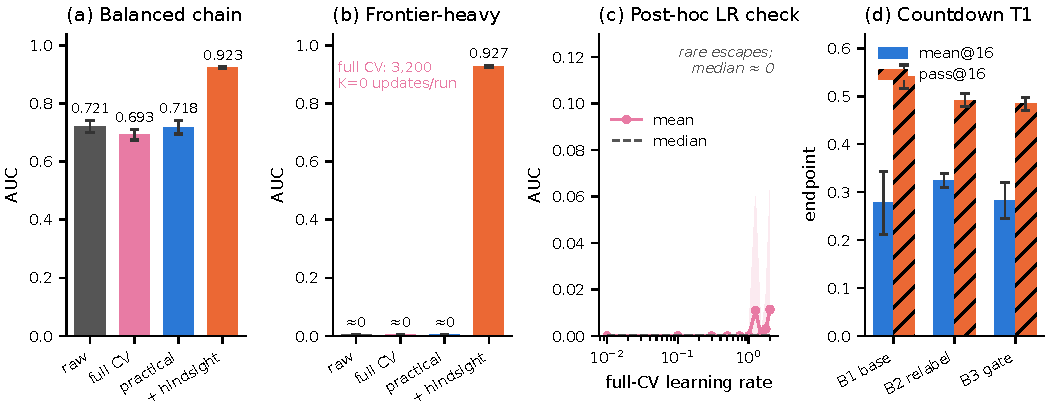
\includegraphics[width=\linewidth]{figures/fig2_ladder}
\caption{\textbf{Local estimator controls and sensitivity.} Panels (a--b)
compare the three MaxRL variants and practical+hindsight at a common
3,200-group budget over 20 paired seeds. Full CV assigns negative
coefficients and invokes the update callback on every frontier all-fail
group but does not reliably bootstrap;
hindsight does. Panel (c) is a post-hoc full-CV learning-rate sensitivity:
rare large-step escapes do not form a reliable regime. Panel (d) shows the
three-seed legacy per-trace Countdown mean/coverage trade; B3 is the unintended moderate
gate operating point. All values load from committed JSON artifacts.}
\label{fig:ladder}
\end{figure}

\paragraph{6.1 Exact-score chains: what comes from allocation, dose,
and direction?} On the tabular shared-skill chain, uniform sampling reaches
\(0.650\) AUC and the posterior \(\nu_N\) teacher reaches \(0.728\). A
five-seed historical control battery reaches \(0.798\)--\(0.800\) under
double learning rate or the random-target placebo, \(0.832\) under
live-gradient replay, and \(0.869\) under verified relabeling. The
hindsight-minus-replay difference is \(+0.037\) in all five paired seeds.
Because update counts/norms were not logged and the random-target arm was
not exactly re-verified, these arms suggest---but do not causally
decompose---dose and direction. The order-agnostic \(p(1-p)\) teacher
forfeits the allocation gain (\(-.007\) versus uniform), whereas \(\nu_N\)
adds \(+.078\), five of five paired.

A true-pass-rate, no-floor, \(\gamma{=}4\) utility benchmark reaches
\(0.8885\); the full posterior-plus-recycling stack reaches \(0.8895\), and
true-pass-rate allocation plus recycling reaches \(0.8935\). These nearby
numbers compare different interventions and do \emph{not} establish a
sequential allocation ceiling. In a matched \(\gamma{=}1\) sampler
comparison, the true-rate oracle reaches \(0.8511\) versus \(0.7278\) for
the posterior teacher, showing the value of exact rates on this chain under
that protocol. Relabeling also retains an incremental effect at the
true-rate operating point. All arms finish within \(.027\), so the
interventions mainly buy time-to-ceiling in this reusable fixed pool.
\takeaway{Coefficient-mass allocation helps on the chain. A historical
placebo battery is consistent with a substantial extra-update contribution,
and hindsight remains \(+.037\) above live-gradient replay, but incomplete
update logging prevents a causal dose--direction decomposition.}

\paragraph{6.2 Can a negative-only all-fail update bootstrap the frontier?
(20 paired seeds; exact-score tabular testbed).} This is the missing
estimator control suggested by the MaxRL taxonomy. We compare raw \(H_N\),
full-CV \(C_N\), practical \(D_N\), and practical plus exact prefix
relabeling under identical uniform task draws, rollout random numbers, common
learning rate \(0.5\), and \(3{,}200\) groups of \(N=16\). The
frontier-heavy pool contains levels 5--12 and has maximum initial pass rate
\(10^{-5}\). Full CV assigns nonzero negative coefficients and invokes
\texttt{policy.update} on every one of the 3,200 all-fail groups per run,
yet does not reliably bootstrap: its AUC
is \(1.74\times10^{-6}\) (reported as \(0.000\)), comparable to raw and
practical. Verified hindsight uses \(158.0\) relabeled groups on average and
reaches \(0.9269\pm0.0032\) AUC / \(0.9788\pm0.0006\) final, winning all
20 paired seeds. On the balanced pool, full CV reaches
\(0.6934\pm0.0189\), practical reaches \(0.7183\pm0.0231\), and practical
is higher by \(.0249\) in 16/20 paired seeds; hindsight reaches
\(0.9227\pm0.0035\).

This is a budget- and testbed-specific negative result for the alternative,
not an impossibility theorem. A post-hoc full-CV learning-rate sweep finds
one of 20 seeds exceeding final pool mean \(.1\) at each of rates 1.25 and
2.0, none at the other eight rates, and median AUC approximately zero throughout (best mean
AUC \(.011\)). These rare, non-monotone escapes remain far below hindsight
and do not define a reliable operating region. The primary comparison used
no estimator-specific tuning. In an earlier five-seed regime control, uniform,
DAPO-style redraw, and posterior allocation also round to zero, whereas
uniform+recycling and teacher+recycling have similar observed AUCs
(\(.931\) and \(.928\)). Thus the
evidence supports a narrow statement: in this frontier, redistributing
negative score mass did not replace a verified positive anchor at the
matched budget.

The common-rate comparison is not a fair performance ranking of differently
scaled estimators. We therefore replay an identical uniform task sequence,
group size, and rollout-uniform stream for practical MaxRL, GRPO, and RLOO.
Learning rates are selected by a one-standard-error rule on 10 tuning seeds
and evaluated on 20 separate held-out seeds. Practical MaxRL reaches
\(0.9889\pm0.0089\) evaluation-grid AUC, GRPO \(0.9841\pm0.0121\), and
RLOO \(0.9869\pm0.0099\); the largest mean separation is \(.0048\). On
binary mixed groups, these estimators' coefficient vectors are positive
scalar multiples of the same centered reward vector, with a
\(K\)-dependent scale. This local near-ceiling control shows why common-rate
comparisons can exaggerate scale differences. Its ordering is specific to
the parameterization-dependent one-standard-error rule, so we do not treat
it as an intrinsic estimator ranking or evidence about the adaptive
neural-maze interaction.
\takeaway{Full CV proves that nonzero coefficients can reach the policy
update callback on all-fail samples; the 20-seed control shows that this
branch does not reliably unlock this
frontier, while verified relabeling does. Fixed-schedule tuning also puts
three collinear binary-reward estimators within \(.005\) AUC here.}

\paragraph{6.3 Historical neural maze: legacy utility/recycling and a
descriptive estimator-associated coverage pattern (1.26M parameters).}
The matched-wall-clock suite contains
roughly 30 historical runs across sampler, estimator, relabel dose, and
utility-form ablations. Its wall-clock limit defines each run's stopping
budget, while the reported AUC integrates over that run's optimizer-step
grid. The primary method comparison is three paired
warm-start blocks: the legacy frontier-ALP teacher plus dense per-trajectory
positive-only recycling reaches
\(0.252\pm0.006\) final / \(0.229\pm0.010\) AUC, versus uniform practical
MaxRL at \(0.230\pm0.018\) / \(0.211\pm0.014\); each block's final and AUC
difference is positive. In the separate teacher-only pairs, frontier-ALP
arms log \(1.2\)--\(1.4\times\) more optimizer steps per wall-clock budget.
The cause is unresolved: generated actions/tokens and runtime composition
were not logged, and zero-weight-group counts do not support attributing the
difference to skipped backward passes. At a common step count, teacher-only
adds \(.006\) AUC with mixed paired signs, whereas teacher+recycling remains positive in all three
blocks. The equal-step result attenuates the clock-matched effect and flips
one paired sign, suggesting that runtime composition contributes; with
three blocks and no generated-token counts, its share is unidentified. The
positive-only recycler is the more stable residual pattern in this archive.
These runs use neither the exact \(\nu_N\) sampler nor a
common-destination contrastive group and therefore do not validate
Algorithm~\ref{alg:frontiermax}.

For the estimator comparison, the frozen selected endpoint cohort contains
five practical-MaxRL-labelled runs (two uniform, three frontier-ALP) and four
GRPO-labelled runs (three uniform, one frontier). Their
\(\Delta\passat{8}\) values are all positive for the MaxRL-labelled runs and
all negative for the GRPO-labelled runs. This is an informative historical
pattern, but sampler composition is unbalanced and seed/warm-start blocks
recur. Neither the earlier unrestricted calculation nor its
sampler-stratified replacement has a valid exchangeable reference
distribution; both are withdrawn as inferential claims. The suite supports
an \emph{estimator-associated} coverage separation across selected
curriculum variants, not a causal teacher-by-estimator interaction. A
balanced factorial with frozen realized schedules remains required.

The CPU utility-form artifact compares exact \(\nu_N\), the legacy frontier
form, and a \(p(1-p)\) slice. The corresponding three-seed maze verdict file
and raw utility-form logs are not vendored, so the prior maze ranking is
withdrawn. We therefore claim the activity profile and peak, not a
universally optimal within-frontier ranking. The single-checkpoint inference sweep is retained
as a secondary diagnostic in Appendix~\ref{app:rungs}: GRPO leads at
\(\passat{1}\), the summed-coverage curves cross near \(k=4\), and practical
MaxRL leads at larger \(k\).

\paragraph{6.4 Exploratory localization across the maze archive.}
Figure~\ref{fig:bands} uses a frozen list of four GRPO and 18 nonempty
practical-MaxRL logs. These are heterogeneous ablations, not 22 independent
replicates of one treatment. The exact cohort and explicitly unrecorded
metadata are committed in \texttt{fig8\_maze\_run\_registry.csv}.
Descriptively, GRPO-labelled
\(\passat{8}\) loss concentrates on levels 1--3 while \(\passat{1}\)
there rises; practical-MaxRL logs are approximately flat on levels 1--3 and
gain more on levels 4--6. The GRPO coverage gap
\(\overline{\passat{8}-\passat{1}}\) erodes early: more than half of its
endpoint change appears by one quarter of each run's wall-clock budget in all
four GRPO-labelled logs. Sparse and
dense legacy positive-only variants suggest that dose changes whether gains are banked
in mean success or multi-sample coverage, but that comparison is likewise
exploratory.

\begin{figure}[t]
\centering
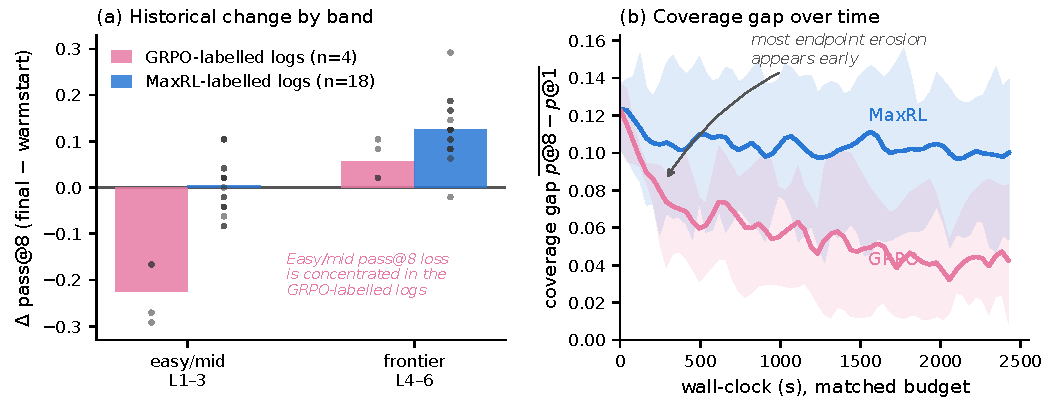
\includegraphics[width=\linewidth]{figures/fig8_bands}
\caption{\textbf{Exploratory maze localization (matched wall-clock).}
\emph{(a)} \(\Delta\passat{8}\) by difficulty band for a frozen archive
of four GRPO and 18 heterogeneous practical-MaxRL runs. Dots are runs, not
independent factorial replicates. \emph{(b)} Mean and range of the coverage
gap \(\overline{\passat{8}-\passat{1}}\) over wall-clock. The figure
localizes a historical association; it carries no pooled permutation test.}
\label{fig:bands}
\end{figure}
\takeaway{The neural archive suggests estimator-associated coverage
behavior and locates it in the easy/mid band, but it uses legacy allocation
and recycling and its unbalanced adaptive schedules do not identify an
interaction or validate the proposed loop.}

\paragraph{6.5 When does allocation \emph{not} pay? (IsaacLab legged
locomotion, one-seed pilot).} A 5-arm Anymal-C rough-terrain pilot
(reported by an independent team from a co-designed protocol; raw logs are
not included here; App.~\ref{app:rungs}) is consistent with its anticipated
null: on a
terrain grid where every level is learnable at budget, the stock greedy
curriculum beats the frontier teacher outright (mean pass .372 vs.\
.278). One seed cannot establish a regime rule; it supplies a boundary
hypothesis for replication: when the pool is learnable throughout at the
deployed budget, breadth may dominate frontier focus.

\paragraph{6.6 What does a curriculum add beyond task spread? (Gymnasium
control --- binary-success RLVR on classic control; official-task
currency).}
All arms train on \emph{binary task success} (MountainCar: reach the
flag; CartPole: survive 400) --- the classic-control analogue of a
verifier reward. The \textbf{target-only} arm remains empirically frozen in
the committed runs: no hardest-task success is observed, and any all-fail
group has exactly zero weights under the deployed practical estimator. The
artifacts do not record every parameter update, so we do not elevate that
empirical freeze to a universal impossibility claim. The gated full stack
under the identical reward reaches
\textbf{1.000$\pm$0.000 on both official tasks} (3 seeds,
Fig.~\ref{fig:gym}). A dense-reward control confirms the zero is a
property of sparse verifier-style reward (REINFORCE on CartPole's
native reward solves it; App.~\ref{app:rungs}). Attribution at a
common horizon: uniform-over-bins task spread supplies most of the
effect (existence of a gradient). Recycling without allocation plateaus
below ceiling on CartPole, while on MountainCar its final success reaches
ceiling but later than the gated stack. Relative to uniform, the full gated
stack is associated with speed and stability: roughly \(3\times\) faster to MountainCar hard-task
0.9 and, for common-280 hard-task AUC, about \(6\times\) smaller cross-seed
sample SD than uniform on both tasks. A methods note from this control: our
own first version used per-bin
task-partitioned policy parameters and reproduced the known failure
(0.000 in every arm). In this Gym setting, the curricula required shared
parameters to transfer competence across bins.

\takeaway{In this control, task spread creates the first usable practical-
estimator update, and shared parameters let that update transfer. Full CV
is a separate all-fail baseline rather than part of this claim.}

\paragraph{6.7 GSM8K 360M: a two-seed legacy-utility treatment-delivery pilot.}
The 50-step \(2\times2\) study is much smaller than the MaxRL baseline's
large-model evidence and is not confirmatory. In the registered seed,
GRPO+teacher ends below GRPO uniform by \(-.027\) mean@4 and \(-.048\)
\(\passat{4}\); its second-half change (\(.096\to.093\)) is smaller than
fixed-checkpoint evaluation noise. In seed 2 the endpoint differences have
the same signs (\(-.007\), \(-.026\)), but GRPO+teacher climbs throughout.
Thus the registered regression shape occurs in one of two seeds. The
\(.0094\) repeated-evaluation SD estimates generation noise for one
checkpoint; it is not training-seed uncertainty and is not used as a
replication test.

The treatment itself uses the historical \((1-q^N)q\) utility rather than
the derived \(\nu_N\) profile and is weak and confounded. Teacher cells sample with
replacement, so repetition differs from uniform; the replacement-matched
control is incomplete. Across 3,200 groups and 7,473 prompts, only 2,561
prompts (34.3\%) are visited: 0.428 group visits per pool prompt, or 1.25
visits per visited prompt. The posterior utility remains nearly flat.
Teacher and uniform sampled-dead fractions have similar observed run means
\(.66\)--\(.67\); the more negative seed has a slightly stronger minimum
separation. Under practical MaxRL, the single recorded teacher run finishes at
\(.102\) versus \(.108\) for uniform, a null at this budget. We retain the
pilot because it diagnoses posterior starvation and treatment delivery, not
because it identifies a curriculum-by-estimator interaction. A
replacement-matched, steering-controlled, multi-seed study with a frozen
evaluation harness is required.
\takeaway{At this scale the legacy-utility prompt-level posterior is starved;
the factorial interaction and the proposed sampler remain unresolved.}

\begin{figure}[t]
\centering
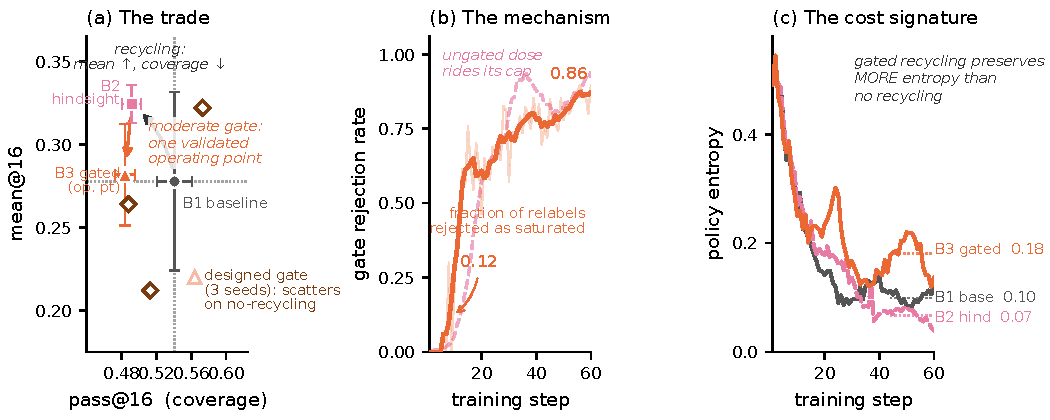
\includegraphics[width=\linewidth]{figures/fig7_sharpening}
\caption{\textbf{Legacy per-trace Countdown sharpening and gate evidence.}
\emph{(a--b)} Three-seed endpoints for saturated tier 1 and frontier tier 2.
Ungated legacy recycling (B2) raises mean success and lowers \(\passat{16}\).
The unintended moderate gate setting (B3) returns frontier-tier coverage
but not saturated-tier coverage. The corrected stronger setting is shown as
one seed, not as an error bar or a dose-response curve.
\emph{(c)} In-run rejection and entropy telemetry for one B3 seed.}
\label{fig:sharpening}
\end{figure}

\paragraph{6.8 Countdown: a legacy per-trace recycler raises the mean while
reducing coverage.}
The first pool was too easy: its baseline reached 76--94\% of a
random-guesser bound, so registered allocation and creation improvements
returned null. It nevertheless exposed the relevant metric mismatch:
relabeling improved mean@16 while reducing \(\passat{16}\). We rebuilt the
pool with operand permutation, parenthesization, exact division, and a
headroom screen, then ran no recycling (B1), ungated recycling (B2), and a
destination gate (B3) for three paired seeds. These historical runs assign
each admitted trace its own achieved target within a uid group and use
positive-only relabeled updates. They therefore have mixed conditioning and
do not instantiate Algorithm~\ref{alg:frontiermax}'s one-destination
\(K'\)-of-\(N\) contrast. The results below describe that legacy recycler,
not the proposed destination-group estimator.

The three-seed aggregate endpoint pattern recurs on the rebuilt pool. On
tier 1, B1 to B2 changes
mean@16 from \(.278\pm.066\) to \(.324\pm.014\) and \(\passat{16}\) from
\(.541\pm.024\) to \(.492\pm.013\). On frontier tier 2, mean changes from
\(.117\pm.037\) to \(.143\pm.017\), while coverage changes from
\(.274\pm.018\) to \(.237\pm.079\). These are aggregate mean and sample-SD
summaries; the underlying three per-seed endpoint rows are not vendored, so
we do not claim a per-seed direction. Only two of the three tier-2 pairs retain
checkpoint trajectories. Both have higher recycled-arm mean at step 30,
but their coverage paths differ: one is lower by step 15 and the other only
by step 45. We therefore make no general timing or early-stopping claim.

This pattern is not a consequence of coefficient mass alone. The legacy
achieved-destination selector samples destinations from the policy's own occupancy,
so already-reachable outcomes are replayed more often; repeated selection is
size-biased toward them relative to the task distribution. Exact
verification preserves label validity but not destination balance. Related
concentration mechanisms motivate GoalGAN, CHER, Skew-Fit, GCSL, and HIPI
\citep{goalgan,cher,skewfit,gcsl,eysenbach}. We retain this as a direct
measurement of a legacy RLVR recycler's large-\(k\) coverage cost. It does
not establish the behavior of shared-anchor, contrastive relabeling.

\paragraph{6.9 Destination saturation is promising for the legacy recycler,
but the gate is not yet a validated dial.} At the unintended three-seed B3 operating point, tier-2
coverage is \(.279\pm.024\), close in point estimate to B1's
\(.274\pm.018\), while mean@16 is \(.133\pm.008\), retaining roughly 60\%
of B2's mean-increment point estimate. On saturated tier 1, however, B3 is
\(.282\pm.037\) mean / \(.484\pm.014\) coverage: it removes most of B2's mean change without
restoring B1 coverage. A decay-math bug made these B3 runs weaker than the
intended gate and turns them into an unintended moderate operating point.

The corrected stronger gate has only one seed: tier 1 \(.220/.564\)
(mean/coverage) and tier 2 \(.083/.238\). It improves saturated-tier
coverage while reducing both frontier metrics; together with B1--B3, this
does not establish monotonicity or a Pareto frontier. One-run telemetry is
mechanistically consistent with saturation admission---rejection rises from
roughly \(.12\) to \(.85\) as destinations become reachable, and B3 retains
more entropy than B1 in that seed---but it is not independent replication.
The supported conclusion is narrower: destination pass rate is a plausible
admission variable for this legacy relabeler, and one moderate setting
returns the frontier-coverage point estimate near baseline. This is not a
prespecified noninferiority result or evidence for the shared-anchor algorithm.
A corrected fixed-decay multi-seed sweep with a prespecified coverage
noninferiority test is required before recommending a gate strength.
\takeaway{Recycling-induced sharpening is a three-seed aggregate endpoint
pattern for the legacy per-trace recycler. Its gate has a promising frontier operating point, but
neither result validates the proposed common-destination algorithm.}

\section{Related work}

\textbf{Group estimators and difficulty weighting.}
GRPO originates in DeepSeekMath, while RLOO revisits leave-one-out
REINFORCE-style optimization for language-model alignment
\citep{grpo,rloo}. MaxRL derives a family of likelihood objectives and
unbiased finite-sample estimators \citep{maxrl}; Mroueh independently
analyzes GRPO's effective loss, calibration, and success amplification
\citep{mroueh}. SC-SDPO and A-GRAE make estimator--difficulty weighting
explicit for GRPO-style training \citep{scsdpo,agrae}. Our distinction is
finite-group and implementation-specific: raw, full-control-variate, and
drop-constant-group MaxRL have different coefficient-mass profiles, and the
last admits the exact factorization in Eq.~\ref{eq:factor}. We then use that
profile as a data-selection score and audit \(\passat{k}\), rather than
proposing another population objective.

\textbf{Curricula and response-budget allocation.}
RLVR curricula include bucket bandits (DUMP), scalar difficulty controllers
(AdaRFT), category bandits (SEC), dynamic filtering (DAPO, GRESO), and
learnability-based prompt selection (SFL, LILO)
\citep{dump,adarft,sec,dapo,greso,sfl,lilo}. LILO prioritizes success
variance \(p(1-p)\); Online Difficulty Filtering independently derives a
policy-improvement lower bound favoring intermediate-difficulty tasks under
GRPO \citep{odf}. At \(N=2\), our normalized practical-MaxRL mass reduces
to the same algebraic score; for \(N>2\), it is group-size- and
estimator-specific. Reinforce-Ada reallocates a fixed batch-level response
budget across prompts, including sequential allocation based on successes,
while leaving macro prompt selection fixed \citep{reinforceada}. Our
teacher instead changes future prompt-group selection at fixed \(N\).
Proposition~\ref{prop:alloc} is only the fixed-rate one-step allocation
problem, not a general optimality claim.

\textbf{Goal selection and hindsight proposal shift.}
HER is explicitly off-policy \citep{her}. GoalGAN generates
intermediate-difficulty goals; HGG balances achievability against target
relevance; CHER schedules relabel goals using proximity and diversity; and
Skew-Fit uses inverse-density skew to improve state coverage
\citep{goalgan,hgg,cher,skewfit}. GCSL derives an off-policy lower bound,
while HIPI derives a corrected inverse-inference relabel law
\citep{gcsl,eysenbach}. Difficulty- and coverage-aware relabel admission is
therefore established. Our gate belongs to this family: the practical
estimator's saturated endpoint motivates destination pass rate as the
admission variable, but its threshold is tuned. The distinct empirical
question is whether this admission preserves large-\(k\) coverage.

\textbf{Hindsight in language and verifiable-reward loops.}
CodeIt and proof-tree relabeling reuse verified outputs for program synthesis
and formal mathematics \citep{codeit,minimo}. HiR directly rewrites failed
instruction-following rollouts into hindsight instructions for RL; HSL and
AgentHER relabel language-agent trajectories for supervised or preference
training \citep{hir,hsl,agenther}. LfH proposes hindsight instructions for
VLA post-training, and ZipRL replays hindsight responses in multi-turn
training \citep{lfh,ziprl}. Thus language-agent relabeling is prior art.
Related work also documents precision--coverage tension in RLVR and
self-training \citep{yue,cui,yuan,starcross}. Our focus is the conjunction:
to our knowledge, no prior method (i) derives the exact finite-\(N\)
coefficient-mass profile of deployed drop-constant-group MaxRL, (ii) uses
that profile for cross-prompt allocation while using its saturation endpoint
for destination admission, and (iii) evaluates the relabeling policy with
large-\(k\) coverage. This conjunction is the proposed method; the current
neural and LLM archives instantiate neither piece together and therefore do
not provide end-to-end validation.

\section{Limitations and negative results}\label{sec:limits}

\paragraph{Identification and scale.}
The maze archive reuses warm starts, mixes samplers, and uses a legacy
utility/recycler, so it supplies a descriptive estimator association, not an
interaction estimate or method validation. GSM8K is a
50-step 360M-parameter pilot with one or two seeds per cell, a replacement
confound, and weak delivered steering. IsaacLab has one seed. The corrected
strong gate has one seed. None supports a broad safety or scale claim; the
required studies are an exact-\(\nu_N\), shared-anchor maze factorial; a
replacement-matched multi-seed LLM factorial; independent locomotion seeds;
and a corrected shared-anchor multi-seed Countdown gate sweep.

\paragraph{Estimator activity is not task transfer.}
\(\nu_N\) exactly scales a prompt-local expected update, not its norm, SNR,
cross-task benefit, or long-horizon value. The full-CV control is likewise
local: under a common learning rate and matched budget, negative-only
updates do not reliably unlock the exact-score chain. The post-hoc
learning-rate sweep has one of 20 threshold crossings at two of ten rates
and none elsewhere, so this result neither proves that full CV always fails
nor supplies a reliable operating region. A separate fixed-schedule,
held-out-tuned tabular control puts practical MaxRL, GRPO, and RLOO within
\(.005\) evaluation-grid AUC, but does not identify the neural curriculum
interaction.

\paragraph{Hindsight is semantically verified but generally off-policy.}
The exact-score chain and corrected NumPy adapters instantiate the proposed
shared-destination contrast; historical maze and Countdown runs do not. An
exact verifier removes label error, not source-to-destination proposal
shift. Same-group destination choice adds selection dependence, and our
behavioral placebo battery does not estimate that bias. Cross-fitted
destination selection, fresh-destination comparisons, and proposal
diagnostics are open. Noisy or learned verifiers would add a second error
source not studied here.

\paragraph{Pool support and shared transfer remain boundary hypotheses.}
The committed Jugs feasibility screen finds one shallow learnable stratum and
zero observed success in deeper strata at its evaluation budget, despite
nonzero relabel yield. The planned multi-arm training results are not
vendored, so we do not infer a fixed point, entropy collapse, or a causal
support requirement from that suite. No exact-score streaming control is
vendored either, so the role of reusable cross-task transfer remains open.

\paragraph{Negative transfers and artifact limits.}
One longer-duration maze run did not solve the deep frontier. Project notes also describe
single-seed \(\gamma\)-concentration, a \((1-p)\)-tilted utility, and teacher
posterior inflation from relabels, but their complete verdict artifacts are
not vendored and we draw no quantitative conclusion from them. A historical
adaptive-truncation result is withdrawn because its implementation dropped
the \(K=0\) control variate; the corrected subset estimator has exact tests
but no committed schedule-matched empirical comparison. Historical figures were assembled before a
single frozen run manifest existed; a checked-in registry now freezes the
Figure~\ref{fig:bands} cohort, while missing raw LLM and multi-seed
corrected-gate artifacts prevent stronger reanalysis. The new estimator-control artifacts
record seeds, commands, versions, source hashes, paired contrasts, and
matched budgets, but the same standard must be applied prospectively to all
neural runs.

\section{Conclusion}
The practical drop-constant-group MaxRL estimator has an exact finite-group
activity profile, and its expected update factorizes into that scalar and a
task-specific score separation. This result guides where allocation can
seek contrast, while the three-estimator taxonomy prevents overextending it:
full control variates can assign nonzero coefficients to all-fail groups,
and hindsight changes the
data proposal rather than merely the coefficient. The new 20-seed control
shows that negative-only coefficients do not reliably bootstrap one extreme
frontier at the matched budget, whereas exact shared-prefix relabeling does.
Legacy Countdown then shows a possible cost: its per-trace positive-only
recycler raises mean success while reducing multi-sample coverage. Because
the neural and LLM runs predate both defining pieces of the proposed loop,
end-to-end method validation remains open. The practical recommendation is
therefore modest:
state the exact estimator implementation, audit finite-group activity,
separate local activity from transfer, and report \(\passat{k}\) alongside
the mean.

\begin{thebibliography}{99}\small
\bibitem[Tajwar et al.(2026)]{maxrl} Tajwar, F., Zeng, G., Zhou, Y., Song,
Y., Arora, D., Jiang, Y., Schneider, J., Salakhutdinov, R., Feng, H., and
Zanette, A. Maximum Likelihood Reinforcement Learning. \emph{ICML}, 2026.
\bibitem[Ahmadian et al.(2024)]{rloo} Ahmadian, A., Cremer, C., Gall{\'e},
M., Fadaee, M., Kreutzer, J., Pietquin, O., {\"U}st{\"u}n, A., and Hooker,
S. Back to basics: revisiting REINFORCE-style optimization for learning from
human feedback in LLMs. \emph{ACL}, 2024, pp.~12248--12267.
\bibitem[Shao et al.(2024)]{grpo} Shao, Z., Wang, P., Zhu, Q., Xu, R., Song,
J., Bi, X., Zhang, H., Zhang, M., Li, Y.~K., Wu, Y., and Guo, D.
DeepSeekMath: pushing the limits of mathematical reasoning in open language
models. arXiv:2402.03300, 2024.
\bibitem[Mroueh(2025)]{mroueh} Mroueh, Y. Reinforcement learning with
verifiable rewards: GRPO's effective loss, dynamics, and success
amplification. arXiv:2503.06639, 2025.
\bibitem[Liu et al.(2026)]{scsdpo} Liu, Z., Cao, Y., Chen, J.,
Honavar, V.~G. Restoring the sweet spot: pass-rate weighted
self-distillation for LLM reasoning. arXiv:2605.27765, 2026.
\bibitem[Yue et al.(2025)]{yue} Yue, Y., et al. Does RL really
incentivize reasoning capacity in LLMs beyond the base model?
\emph{NeurIPS} (oral), 2025.
\bibitem[Yuan et al.(2026)]{yuan} Yuan, S., et al. Understanding
diversity collapse in RLVR via the lens of overtraining.
arXiv:2606.15455, 2026.
\bibitem[Cui et al.(2025)]{cui} Cui, G., et al. The entropy mechanism of
RL for reasoning language models. arXiv:2505.22617, 2025.
\bibitem[Wang et al.(2025)]{dump} Wang, Z., Cui, G., Li, Y.-J., Wan, K., Zhao, W. DUMP: automated
distribution-level curriculum learning for RL-based LLM post-training.
arXiv:2504.09710, 2025.
\bibitem[Shi et al.(2026)]{adarft} Shi, T., Wu, Y., Song, L., Zhou, T., Zhao, J. Efficient
reinforcement finetuning via adaptive curriculum learning.
\emph{TMLR}, 2026. arXiv:2504.05520.
\bibitem[Bae et al.(2026)]{odf} Bae, S., Hong, J., Lee, M.~Y., Kim, H.,
Nam, J., and Kwak, D. Online difficulty filtering for reasoning oriented
reinforcement learning. \emph{EACL}, 2026, pp.~700--719.
\bibitem[Chen et al.(2025)]{sec} Chen, X., et al. Self-evolving
curriculum for LLM reasoning. arXiv:2505.14970, 2025.
\bibitem[Foster et al.(2025)]{lilo} Foster, T., Sims, A., Forkel,
J., Foerster, J. LILO: learning to reason at the frontier of
learnability. \emph{NeurIPS}, 2025.
\bibitem[Yu et al.(2025)]{dapo} Yu, Q., et al. DAPO: an open-source LLM
reinforcement learning system at scale. \emph{NeurIPS}, 2025.
\bibitem[Xiong et al.(2025)]{reinforceada} Xiong, W., et al.
Reinforce-Ada: an adaptive sampling framework under non-linear RL
objectives. arXiv:2510.04996, 2025.
\bibitem[Zheng et al.(2025)]{greso} Zheng, H., et al. Act only
when it pays: efficient reinforcement learning for LLM reasoning via
selective rollouts (GRESO). \emph{NeurIPS}, 2025.
\bibitem[Andrychowicz et al.(2017)]{her} Andrychowicz, M., et al.
Hindsight experience replay. \emph{NeurIPS}, 2017.
\bibitem[Florensa et al.(2018)]{goalgan} Florensa, C., Held, D., Geng,
X., Abbeel, P. Automatic goal generation for reinforcement learning
agents. \emph{ICML}, 2018.
\bibitem[Ren et al.(2019)]{hgg} Ren, Z., Dong, K., Zhou, Y., Liu, Q.,
Peng, J. Exploration via hindsight goal generation. \emph{NeurIPS},
2019.
\bibitem[Fang et al.(2019)]{cher} Fang, M., Zhou, T., Du, Y., Han, L.,
Zhang, Z. Curriculum-guided hindsight experience replay.
\emph{NeurIPS}, 2019.
\bibitem[Pong et al.(2020)]{skewfit} Pong, V.~H., Dalal, M., Lin, S.,
Nair, A., Bahl, S., Levine, S. Skew-Fit: state-covering self-supervised
reinforcement learning. \emph{ICML}, 2020.
\bibitem[Eysenbach et al.(2020)]{eysenbach} Eysenbach, B., Geng, X.,
Levine, S., Salakhutdinov, R. Rewriting history with inverse RL:
hindsight inference for policy improvement. \emph{NeurIPS}, 2020.
\bibitem[Ghosh et al.(2021)]{gcsl} Ghosh, D., et al. Learning to reach
goals via iterated supervised learning. \emph{ICLR}, 2021.
\bibitem[Xu et al.(2026)]{lfh} Xu, I., Jiang, S., et al. Learning more
from less: reinforcement learning from hindsight. arXiv:2607.09042, 2026.
\bibitem[Zhang et al.(2026)]{hir} Zhang, K., Yao, Q., Liu, S., Zhang, W.,
Cen, M., Zhou, Y., Fang, W., Zhao, Y., Lai, B., and Song, M. Replay failures
as successes: sample-efficient reinforcement learning for instruction
following. \emph{ICML}, 2026.
\bibitem[Li et al.(2026)]{hsl} Li, Z., Wu, G., Wang, Z., Zhang, R., Zhu, W.,
Rossi, R.~A., Morariu, V.~I., and Kil, J. Spinning straw into gold:
relabeling LLM agent trajectories in hindsight for successful
demonstrations. \emph{ICLR}, 2026.
\bibitem[Ding(2026)]{agenther} Ding, L. AgentHER: hindsight experience replay
for LLM agent trajectory relabeling. arXiv:2603.21357, 2026.
\bibitem[Butt et al.(2024)]{codeit} Butt, N., et al. CodeIt:
self-improving language models with prioritized hindsight replay.
\emph{ICML}, 2024.
\bibitem[Poesia et al.(2024)]{minimo} Poesia, G., et al. Learning formal
mathematics from intrinsic motivation. \emph{NeurIPS}, 2024.
\bibitem[Hu et al.(2026)]{ziprl} Hu, Z., Wang, L., Wang, X., et al.
ZipRL: adaptive multi-turn context compression with hindsight response
replay. arXiv:2605.28069, 2026.
\bibitem[Strozzi(2026)]{starcross} Strozzi, I.~L. Teacher-free
self-training amplifies but does not compound: a pass@$K$ crossover on a
free-verifier domain. arXiv:2606.07856, 2026.
\bibitem[Yu et al.(2026)]{agrae} Yu, Z., Chen, Z., Liu, M., et al.
Unveiling implicit advantage symmetry: why GRPO struggles with
exploration and difficulty adaptation. arXiv:2602.05548, 2026.
\bibitem[Rutherford et al.(2024)]{sfl} Rutherford, A., et al. No
regrets: investigating and improving regret approximations for curriculum
discovery. \emph{NeurIPS}, 2024.
\end{thebibliography}

\appendix
\section{Full details for compressed experiment rungs}\label{app:rungs}

Material moved from \S 6 during the page-budget pass. The new estimator
controls and plotted aggregate endpoints are committed with the paper;
historical evidence with incomplete run-level artifacts is identified below.

\paragraph{6.1 control battery (full).} Eight arms, 5 seeds each:
uniform $0.650$, lr$\times 2$ $0.798$, random-target relabels $0.800$,
live-gradient replay $0.832$, true relabels $0.869$, no-floor
$\gamma$-matched oracle $0.8885{\pm}.0015$, full stack
$0.8895{\pm}.0026$, oracle$+$recycling $0.8935{\pm}.0013$. The relabel
hindsight-minus-replay difference ($+.037$) has paired seed spread $\pm.0136$;
its worst seed beats every
placebo's best. Random-target relabels are lower than live-gradient replay
($-.032$, 5/5 seeds) but neutral vs.\ plain lr-doubling. This arm reused a
stale deepest-prefix reward vector, drew destinations from an unseeded RNG,
and did not exactly re-verify them; per-arm update counts and norms were not
logged. It is therefore a historical behavioral placebo, not a clean
dose-matched or direction-isolating control.
Utility-form controls: exact $\nu_N$ $0.728{\pm}.002$ vs.\ legacy
frontier form $0.733{\pm}.015$ (the derived form's payoff has about
$7\times$ smaller sample SD); the $N{=}2$ slice $p(1{-}p)$ is a wash against
uniform ($-.007$, 2/5 wins) where $\nu_N$ carries $+.078$ (5/5). AUC
spread across arms is $9\times$ the final-performance spread.

\paragraph{6.5 IsaacLab protocol.} According to the independent team's
one-seed fixed-grid pilot summary (raw logs are not included here), the five
arms are: frontier teacher, stock
greedy walker, uniform, scripted ramp, no-motion control; fixed-grid
per-level evaluation; Anymal-C rough terrain; one seed, executed by an
independent team against a co-designed protocol. The
teacher's only edge over the greedy walker is a small reported difference at
the hardest evaluated level; no raw logs are available to estimate its noise.

\begin{figure}[t]
\centering
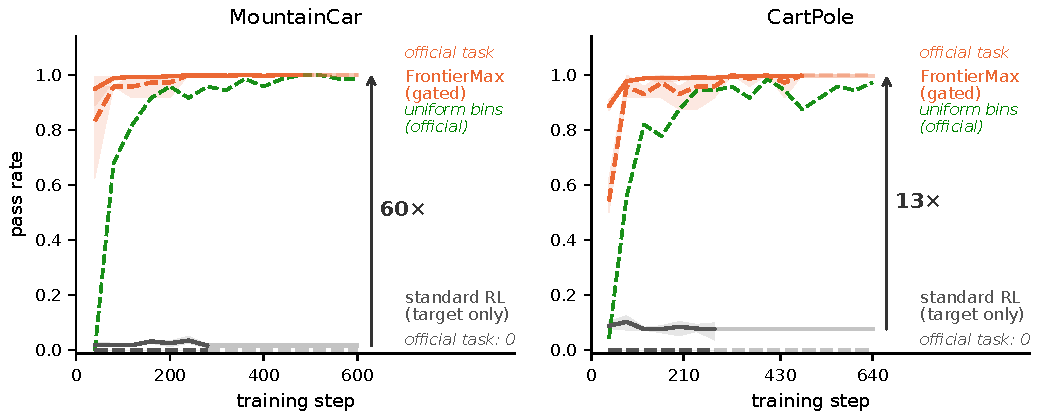
\includegraphics[width=\linewidth]{figures/fig6_gym}
\caption{\textbf{Gym control under binary task-success reward, trained
to plateau (3 seeds).} Solid: mean pass rate across curriculum bins;
dashed: the \emph{official} task (MountainCar flag / CartPole
survive-400). Under the practical drop-constant-group estimator, the
target-only arm (gray) remains empirically frozen; all-fail groups receive
zero weights. A uniform-over-bins control (green) cracks both tasks but
does not end at \(1.000\) in every seed; on MountainCar it is roughly
\(3\times\) slower to hard-task 0.9. The gated FrontierMax stack converges
to $1.000{\pm}0.000$.}
\label{fig:gym}
\end{figure}

\paragraph{6.6 gym control (full).} A dense-reward control using CartPole's
native $+1$/step reward lets vanilla REINFORCE on the same tile policy solve survive-400
($0.963{\pm}0.038$, 3 seeds); MountainCar's native $-1$/step reward
(constant until first success) stays at $0.000$ in all seeds --- the
categorical zero tracks reward sparsity, not the environment.
Attribution at a common 280-step horizon (hard-task AUC): MC $.750 \to$
+recycling $.895 \to$ +teacher $.956$; CartPole $.708 \to .792 \to
.893$; paired teacher increment positive 3/3 seeds on both;
creation-without-allocation plateaus at $0.958$ on CartPole in every
seed while adding the teacher restores $1.000$; teacher speed effect
$3.0\times$ to hard-task $0.9$ ($2.1\times$ to $0.99$ on CartPole).
Earlier random-policy probes and a transition-matched study are documented in
project notes but are omitted here because their raw artifacts are not
vendored.


\begin{figure}[tb]
\centering
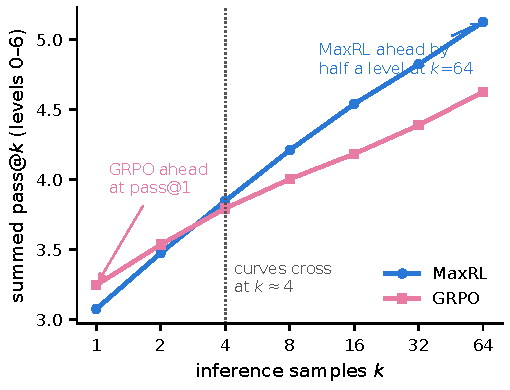
\includegraphics[width=0.55\linewidth]{figures/fig9_ksweep}
\caption{\textbf{Summed maze coverage vs.\ inference samples $k$
(final uniform-arm checkpoints).} In this checkpoint pair, GRPO leads at
$\passat{1}$, the curves cross at $k{\approx}4$, and practical MaxRL leads
by half a level at $k{=}64$. This is a secondary diagnostic, not a general
estimator-selection rule.}
\label{fig:ksweep}
\end{figure}

\paragraph{6.3 inference-efficiency detail.} Convention: smallest $k$
reaching absolute coverage $0.25$, log-interpolated. Artifact
\texttt{efficiency.json} is under
\texttt{curriculum\_maxrl/maze\_gpu/};
Fig.~\ref{fig:ksweep} plots the
summed-coverage crossing. Summed coverage over L0--6: GRPO
$3.24$ vs.\ MaxRL $3.07$ at $\passat{1}$; crossing at $k{\approx}4$.
At $k{=}64$, MaxRL reaches $5.125$ versus GRPO's $4.625$; GRPO's
level-2/4 curves reach $0.875/0.5625$, versus $1.000/0.6875$ for MaxRL.

\paragraph{6.9 secondary read (exploratory).} The committed training
trajectories contain complete entropy and gate-rejection telemetry for one
B1/B2/B3 seed. Over its final 15 steps, mean entropy is $.099/.067/.181$,
respectively. B3's rejection rate trends from roughly $.12$ early to $.86$
late, although the path is not monotone. These one-run telemetry summaries
are mechanistic diagnostics, not independent replication.

\paragraph{6.7 artifact and harness caveats.}
The committed cell trajectories and $\passat{k}$ summary reproduce the
reported training curves and endpoint sweep. The sweep's absolute level is
roughly three times below the trainer validation metric; that harness
discrepancy is unresolved, so only within-sweep contrasts are used.
Posterior-agreement, external-difficulty, response-length, and
prompt-uniqueness diagnostics in the historical postmortem require
non-vendored checkpoints or annotation caches and are therefore not used as
paper evidence.

\paragraph{Jugs feasibility screen (\S\ref{sec:limits}).} The committed
screen evaluates the first 40 tasks per tier from a committed 200-task-per-tier
pool t0--t4 (2--5 jugs, disjoint minimum-move bands), using SmolLM2-360M two-shot generation and
$N=16$. It records
pass@1/pass@16 of $.058/.475$ on t0, $.006/.100$ on t1, and $0/0$ on
t2--t4, while failure-to-relabel yield is $.62$--$.73$ across tiers. No
B1/B2/B3 training-result artifact is present in this checkout. Fixed-point,
entropy, relabel-rate, and gate-rejection claims are therefore omitted until
a run-level snapshot is vendored.

\section{Hyperparameters and compute}\label{app:hparams}

Project notes estimate approximately $230$ A10G-hours for the historical GPU
studies, plus CPU time for the tabular suites; incomplete per-session
accounting prevents reconstructing that total from committed artifacts.
Across 1,188 mixed GSM8K and Countdown telemetry steps, the step-weighted mean
generation fraction is $31.2\%$. Suite-specific raw timing logs are not
vendored, so this aggregate is not a representative per-suite cost breakdown.
Table~\ref{tab:suites} gives the
per-suite configuration and Table~\ref{tab:knobs} the knob inventory
with provenance.

\begin{table}[H]
\centering\scriptsize
\caption{Per-suite configuration. These are the principal settings for each
suite; tuning and evidence status are separated in Table~\ref{tab:knobs}.}
\label{tab:suites}
\begin{tabularx}{\linewidth}{@{}lXXXX@{}}
\toprule
 & chains (\S6.1--6.2) & maze (\S6.3--6.4) & GSM8K (\S6.7) & Countdown (\S6.8--6.9) \\
\midrule
policy & exact-score tabular & 1.26M transformer & SmolLM2-360M & SmolLM2-360M (SFT) \\
allocation/recycler & $\nu_N$ / shared anchor & legacy frontier-ALP / isolated positives & legacy utility / none & legacy utility / per-trace targets \\
rollouts $N$ & 16 & 32 & 16 & 16 \\
groups/step & 1 new; 8 legacy & 8 & 64 & 64 \\
optimizer, lr & SGD; .5 common; tuned 12/16/64 (MaxRL/GRPO/RLOO) & AdamW, $10^{-4}$ & AdamW, $10^{-5}$ & AdamW, $10^{-5}$ \\
budget & 3{,}200 groups & 2{,}400 s clock & 50 steps & 60 steps \\
seeds (headline) & 20 primary; 10 tune + 20 held-out; 5 legacy & 3 selected/arm & 1--2/cell & 3/arm; 1 corrected \\
compute/run & CPU-min & ${\sim}0.7$ A10G-h & ${\sim}20$ A10G-h & ${\sim}6$ A10G-h \\
\bottomrule
\end{tabularx}
\end{table}

\begin{table}[H]
\centering\small
\caption{Teacher and recycler knobs: value, provenance, and measured
sensitivity.}
\label{tab:knobs}
\begin{tabularx}{\linewidth}{@{}p{.20\linewidth}p{.11\linewidth}p{.29\linewidth}X@{}}
\toprule
knob & default & derived or tuned & sensitivity \\
\midrule
profile shape/peak/$N$-dependence & --- & \textbf{derived} (Prop.~1) & the theory claim \\
posterior decay & 0.7 & tuned (V2b) & historical sensitivity; raw artifact absent \\
uniform floor & 0.1 & tuned & historical sensitivity; raw artifact absent \\
$\gamma$ (concentration) & 1 & tuned (V6) & 4 on chains; single-seed maze note, complete verdict artifact absent \\
\texttt{gate\_max\_p} & 0.5 & tuned; saturation-motivated & corrected sweep remains open \\
relabel dose cap & 12 Countdown groups; 16 maze trajectories & suite-specific tuned values & no cap in corrected core; isolated dose response remains open \\
\bottomrule
\end{tabularx}
\end{table}

\section*{Implementation contract and reproducibility}
The finite-group derivations assume i.i.d. rollouts conditional on a requested
task and a binary verifier. Centering statistics are computed over the full
requested group; GRPO uses the sample standard deviation plus the stated
stabilizer. Hindsight selects one common destination for an all-fail group,
rewrites every trajectory to that destination, re-verifies the rewritten
group, and updates only when $0<K'<N$ in the proposed contract. Its teacher
records evidence for the requested task, not the relabeled destination.
GridReach and corrected Countdown regression-test shared-destination
contrast; chain and Gym exercise relabeling without dedicated assertions for
all three contracts. GridReach and Countdown expose only bucket-level
posterior IDs, so their optional gates are bucket rather than exact-destination
estimates. Historical maze and Countdown runs use the legacy semantics stated
in Table~\ref{tab:suites} and are not tests of this contract.

The new finite-group control uses
\nolinkurl{curriculum_maxrl/run_estimator_variants.py} with 20 seeds; the
post-hoc robustness sweep uses
\nolinkurl{curriculum_maxrl/run_fullcv_lr_sensitivity.py}; and the held-out
fixed-schedule comparison uses
\nolinkurl{curriculum_maxrl/run_schedule_matched_estimators.py}.
Structured child random streams keep rollout and schedule randomness
separate across replicates while preserving common random numbers within
paired arms. Their JSON
outputs record seed identities, matched budgets, versions, commands, source
hashes, and paired contrasts. Analytic curves and the new control panels
regenerate from committed code and JSON. Figure~\ref{fig:bands} loads its
22-row frozen registry; other historical neural endpoints are plotted from
available aggregate or run logs, but no single manifest predates all of
those runs. Raw GSM8K, multi-seed corrected-gate, IsaacLab, and complete Jugs
run-level archives remain gaps. The dependency-light
\texttt{frontier\_rl} NumPy core and exact-score testbed are runnable here;
its LLM, IsaacLab, and VLA integrations are prototypes and are not all
end-to-end reproducible in this checkout.

\end{document}
